\chapter{Sensor effects}
\graphicspath{ {./images/} }


\begin{figure}[h]
    \centering
    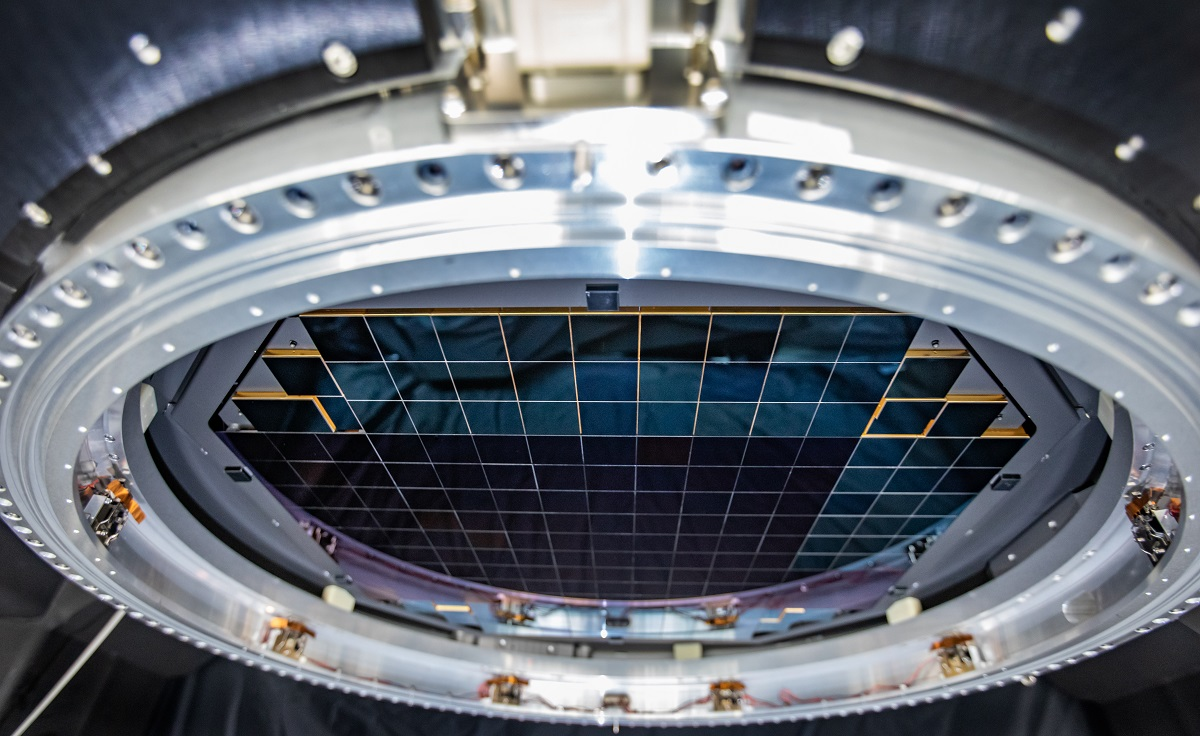
\includegraphics{lsstcam-focalplane-lowres.jpg}
    \caption{LSST full focal plane.}
    \label{fig:focalplane}
\end{figure}

The LSST camera is currently under construction at SLAC National Accelerator Laboratory. Its focal plane (Fig \ref{fig:focalplane}) consists of a mosaic of 189 CCDs and is designed in a highly modular fashion. This design choice facilitates both the ability to assemble and test the rafts in parallel, as well as to quickly isolate any issues or defects without disturbing the rest of the focal plane. The CCDs are arranged on 21 rafts, where each raft is effectively its own autonomous camera \footnote{Roodman, A. Integration and Verification Testing of the LSST Camera, 2018.} with its own matrix of nine CCDs. 




Upon completion, its 3.2 giga-pixel focal plane will make it the largest digital camera ever built. 

\section{Bias and offset corrections in LSST sensors}

Every CCD image that is taken contains a bulk offset that must be subtracted out prior to analysis. This offset level, or bias, can be thought of as a ``zero-point'', and typically contains around 20,000 counts. It is usually measured from the serial overscan region of a single channel in a CCD. The overscan region does not refer to a physical location on the sensor. Rather, this region contains ‘virtual’ pixels that are the result of continuing readout of the sensor after it has reached the last physical pixel in the serial register.

%include image showing CCD architecture and overscan regions

I first looked at bias images to study the performance of various methods of offset correction at the raft, sensor and amplifier level. I then integrated two new offset-correction methods into the EOTest software package, which is a set of acquisition and analysis scripts used to test the electro-optical performance of the Raft Tower Modules (RTMs). A bias image is a zero-second exposure taken with the shutter closed, so it should contain nothing - no light and no dark current - except for the bulk offset level. At the start of my project, the EOTest package had two ways to calculate the offset level. One was to measure the offset as the mean of all the pixels in the serial overscan region, and the other was to fit a low-order polynomial function to the mean per row in the overscan region. I compared these two methods to three other offset-correction methods: calculating the offset as the mean-per-row in the overscan, as a Gaussian process fit and finally as a cubic spline fit to the mean per row in the overscan region. These comparisons can be seen in Fig. []

While the row-by-row correction did the best at characterizing variations in the offset level, it introduced correlated noise of around 10/sqrt(50) ~ 1.4 counts per pixel. The cubic spline fit generally did well at fitting the shape of the mean-per-row without adding a significant amount of extra noise. However its performance varied depending on the sensor vendor (it tended to perform better on e2v sensors), as well as on how well the parameters of the spline fit were adjusted. For example, in some cases, a cubic spline would tend to overfit the data for certain amplifiers, but when the smoothing factor was increased it would come at the cost of losing peaks or dips in the mean-per-row, particularly in the first 50 or so rows. I tried modeling the offset as a gaussian process to see if it would lead to an improvement, but it actually performed worse at fitting the mean-per-row than the cubic spline did. 

I modified the EOTest package to allow the option to apply a mean-per-row or cubic spline offset correction in addition to the existing mean and polynomial fit functions. After carefully studying these methods and applying them to images from TS8, it was decided that the best way to proceed in terms of the current testing software would be to use the mean-per-row method because, even though it introduces slightly more noise, it is significantly more accurate in the lower rows and would suffice for general performance testing. In the end I made this the default offset-correction method for all electro-optical performance tasks in EOTest.

Once the offset level is subtracted and the image is trimmed to remove the overscan region, the next step is to remove the bias. The bias is the pixel-to-pixel structure in the read noise in an image. This structure varies from amplifier to amplifier, as well as across a single amplifier in a CCD. To correct for the bias, a ‘super bias’ is generated for each amplifier by stacking many bias frames that have been offset-corrected and trimmed. I added the functionality in EOTest to be able to stack a set of images according to a statistic (for example, median-stacking or taking a clipped mean of the stacked images), as well as a method to create a ‘super bias’ file, which generates a FITS file containing a super bias for each amplifier for a given raft, sensor and run number. 

Next, I did a study of how well the super bias corrected for the bias level. For a given raft, sensor and run number, I first needed to visually confirm each bias image that would be going into the super bias. I verified all bias images taken during each acquisition mode, which included flat fields, superflats, dark images, quantum efficiency, and an Fe55 source, by plotting serial and parallel projections of each offset-corrected bias image minus the super bias. This amounted to over-plotting the mean of each row/column in every bias minus super bias image against each row/column. I also plotted the mean and sigma over all bias images as a function of row and column. The mean over all biases is expected to be zero and the sigma is expected to be approximately constant, so that bias structure changes would appear as the mean deviating from zero or sigma varying as a function of row or column. Most of the bias images were consistent with what was expected, however there was some peculiar behavior in sigma as a function of row where I observed random oscillations that varied slowly in time. This is something I did not have a chance to investigate thoroughly, but one potential cause to be investigated is banding, which has been observed in some ITL sensors as a row-wise effect where one can see bands going across the image that vary in bias level. 

Projecting the bias in this way revealed an effect called persistence. Several of the corrected bias frames taken during the flat acquisition had mean values as high as 80 counts. Since flat images are taken at increasingly higher exposure times, they detect more light the longer they are exposed. Bias images are taken after every two or three flats, so plotting the timestamp of each flat and bias image showed the outlier bias image as the final bias frame taken during this acquisition. Looking at a projection plot of the flat taken just before this bias image showed the flat to be saturated. It turned out that the excessively high mean value in the outlier bias image was due to charge that had persisted from the previous flat image due to insufficient clearing of the CCD. In this case, more time needed to be allowed between parallel pixel transfers during readout. 

Once all bias images that showed anomalous behavior were removed, I created a super bias for all amplifiers on the sensor from 50 bias images. To study the performance of these super biases, I conducted a ‘ratio test’ using images taken from the superflat acquisition. Superflats were taken in two modes, with low superflats taken to have around 1000 counts, and high superflats having around 50,000 counts. 

The ratio I used to study the super biases was defined as the sum over all bias and offset-corrected low superflats divided by the sum over all bias and offset-corrected high superflats. Because this is essentially a ratio of images, it is immune to any effects like bad pixels or quantum efficiency, which would effectively be divided out. I made a series of two-dimensional histograms of this ratio against the super bias for a number of ITL and e2v rafts. Since the same super bias image is being subtracted from the numerator and the denominator, we would expect the mean of the ratio to be around 1000/50,000 = 0.02 counts, with a sigma of around 0.008. It is also expected that the histogram of the super bias image would have the highest density around zero counts, since the super bias is offset-corrected and should only contain pixel to pixel variations in the noise level. 

The results showed a surprising amount of structure in the super biases, particularly in the ITL sensors. For example, there were ‘clumps’ of points in the super bias that were concentrated in circular lobes at various intervals along the super bias axis. There were also large concentrations of points in the super bias that had values that deviated significantly from zero. On the ratio axis, there were also separate ‘clumps’ of points, most of which were still centered around 0.02, but some of which had slightly lower or higher mean values. After mapping these questionable pixels onto their physical location on the sensor, most either corresponded to bad columns or to the first few columns of an amplifier. This behavior clearly indicates that something is not correct in the way the super bias is being subtracted, and that there may be pixels that should be masked but are being excluded by the current masking selection process in the EOTest code. The e2v sensors were in general more well-behaved, except for a vertical ‘gap’ around a super bias value of zero, where pixels in the super bias were not being plotted. I verified that these super bias images were indeed masked, so the gaps do not seem to be due to bad masking. But I have yet to investigate whether stacking the super bias using a clipped mean rather than the median would fix this issue. 

Lastly, I studied another issue known as bias trending, which was observed by plotting the mean of the imaging section of all bias images in a run over time. Theoretically, a bias image should only contain the offset level, the bias level and the read noise, the last two of which are sub-dominant. This should make the mean stable around 20,000 counts. However this was not the case and there were significant fluctuations in the mean. My work showed that doing a proper bias and offset correction resolved this instability.

\section{Modeling sky brightness in the ImSim package}
\section{Simulating the brighter-fatter effect}

- weak lensing shear requirements, distortion signal from BF

%%% Local Variables: ***
%%% mode: latex ***
%%% TeX-master: "thesis.tex" ***
%%% End: ***
